%%%%%%%%%%%%%%%%%%%%%%%%%%%%%%%%%%%%%%%%%%%%%%%%%%
% Basic setup. Most papers should leave these options alone.
\documentclass[fleqn,usenatbib]{mnras}

% MNRAS is set in Times font. If you don't have this installed (most LaTeX
% installations will be fine) or prefer the old Computer Modern fonts, comment
% out the following line
\usepackage{newtxtext,newtxmath}
% Depending on your LaTeX fonts installation, you might get better results with one of these:
%\usepackage{mathptmx}
%\usepackage{txfonts}

% Use vector fonts, so it zooms properly in on-screen viewing software
% Don't change these lines unless you know what you are doing
\usepackage[T1]{fontenc}

% Allow "Thomas van Noord" and "Simon de Laguarde" and alike to be sorted by "N" and "L" etc. in the bibliography.
% Write the name in the bibliography as "\VAN{Noord}{Van}{van} Noord, Thomas"
\DeclareRobustCommand{\VAN}[3]{#2}
\let\VANthebibliography\thebibliography
\def\thebibliography{\DeclareRobustCommand{\VAN}[3]{##3}\VANthebibliography}


%%%%% AUTHORS - PLACE YOUR OWN PACKAGES HERE %%%%%

% Only include extra packages if you really need them. Common packages are:
\usepackage{graphicx}	% Including figure files
\usepackage{amsmath}	% Advanced maths commands
\usepackage{amssymb}	% Extra maths symbols

%%%%%%%%%%%%%%%%%%%%%%%%%%%%%%%%%%%%%%%%%%%%%%%%%%

%%%%% AUTHORS - PLACE YOUR OWN COMMANDS HERE %%%%%

% Please keep new commands to a minimum, and use \newcommand not \def to avoid
% overwriting existing commands. Example:
%\newcommand{\pcm}{\,cm$^{-2}$}	% per cm-squared

%%%%%%%%%%%%%%%%%%%%%%%%%%%%%%%%%%%%%%%%%%%%%%%%%%

%%%%%%%%%%%%%%%%%%% TITLE PAGE %%%%%%%%%%%%%%%%%%%

% Title of the paper, and the short title which is used in the headers.
% Keep the title short and informative.
\title[Hot Accretion in FIRE]{Galactic Discs Fed Directly by Hot Accretion in FIRE}

% The list of authors, and the short list which is used in the headers.
% If you need two or more lines of authors, add an extra line using \newauthor
\author[\ldots]{
\ldots,$^{1}$\thanks{E-mail: mn@ras.org.uk (KTS)}
\\
% List of institutions
$^1$ \ldots
}

% These dates will be filled out by the publisher
\date{Accepted XXX. Received YYY; in original form ZZZ}

% Enter the current year, for the copyright statements etc.
\pubyear{2020}

% Don't change these lines

\newcommand{\Rcool}{R_{T=10^5 {\rm K}}}
\newcommand{\Mdot}{\dot{M}}
\newcommand{\Rcirc}{R_{\rm circ}} %need better name as R_cool means something else

\begin{document}
\label{firstpage}
\pagerange{\pageref{firstpage}--\pageref{lastpage}}
\maketitle

% Abstract of the paper
\begin{abstract}
\textit{
We compare the contribution of modes of accretion in the FIRE simulation in $L^\star$ halos between cold accretion, hot gas that condenses into clouds and accretes onto the galaxy (``precipitation''), and hot gas that accretes directly onto the galaxy as it cools.
We demonstrate that the primary mode of gas accretion in $L^\star$ halos is hot accretion directly onto the galactic disc.
}

\textbf{Abstract TBD.}
\end{abstract}

% Select between one and six entries from the list of approved keywords.
% Don't make up new ones.
\begin{keywords}
keyword1 -- keyword2 -- keyword3
\end{keywords}

%%%%%%%%%%%%%%%%%%%%%%%%%%%%%%%%%%%%%%%%%%%%%%%%%%

%%%%%%%%%%%%%%%%% BODY OF PAPER %%%%%%%%%%%%%%%%%%

\section{Introduction}
Two modes of hot accretion:
\begin{itemize}
    \item condensation (Maller \& Bullock 2004; Kaufmann, Bullock+09; McCourt+12; Voit+17)
    \item classic CF (Cowie+80; Paper I)
\end{itemize}
\textbf{Intro TBD}

\section{Methods}

% Simulation sample
\textit{
We use four simulations:
m12i\_md\_7100, m12b\_md\_7100, m12f\_core\_7100, m12m\_core\_7100
}
\textbf{Also do massive galaxies?}

% How we select the particles
\textit{
For a given galaxy we select all particles that are in the central galaxy at $z=0$ and in the CGM 1 Gyr prior.
The galaxy is defined as all gas and stars inside $R_{\rm gal} = 4 R_{\star,0.5}$, with an additional density cut of $n_{\rm H} = 0.13$ cm$^{-3}$ for gas.
The CGM is defined as all gas inside $0.1 -1 R_{\rm vir}$.
For each selected particle we retrieve the full history of the particle (including temperature, density, metallicity) throughout the simulation.
}

\textbf{Change the ``inside the galaxy'' radial cut to 0.1 $R_{\rm vir}$ as well and rerun.}

\textbf{The number of IDs that are accreted for m12i is 18554.
However, after removing duplicates, the number of IDs that are tracked is 14703.
Either $\sim20\%$ of the particles split, or this is a symptom of a bug.
Find out which.}


\begin{equation}
    \Rcool \equiv \text{max radius where} T<10^5\,{\rm K}
\end{equation}


the circularization radius $\Rcirc$ is defined via
\begin{equation}
    j = v_{\rm c}(\Rcirc)\Rcirc
\end{equation}
where $j$ is the specific angular momentum and $v_{\rm c}$ is the circular velocity



\section{Results}


\begin{figure}
    \centering
    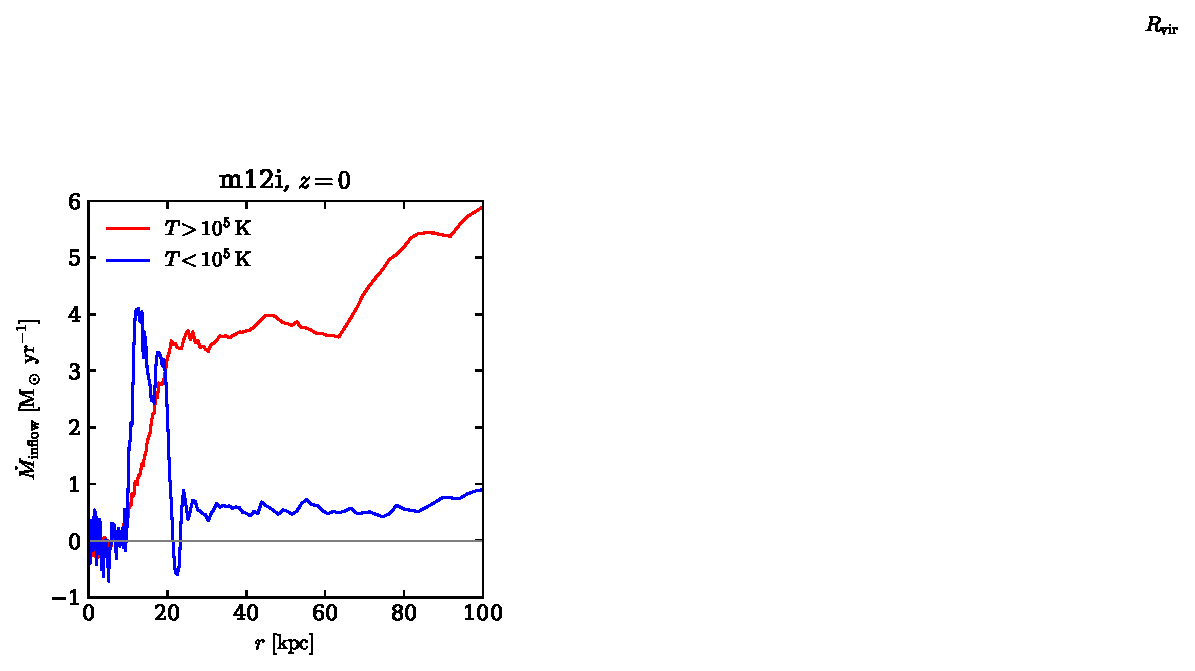
\includegraphics{Mdot_m12i.pdf}
    \caption{
    \textbf{Add images of face-on $z=0$ slice with temperature and velocity arrows.}
    \textbf{Plot too busy. dispersion at disc radii takes to much attention. Change to SFR$(>r)$}
    }
    \label{f:Mdot}
\end{figure}


\begin{figure}
    \centering
    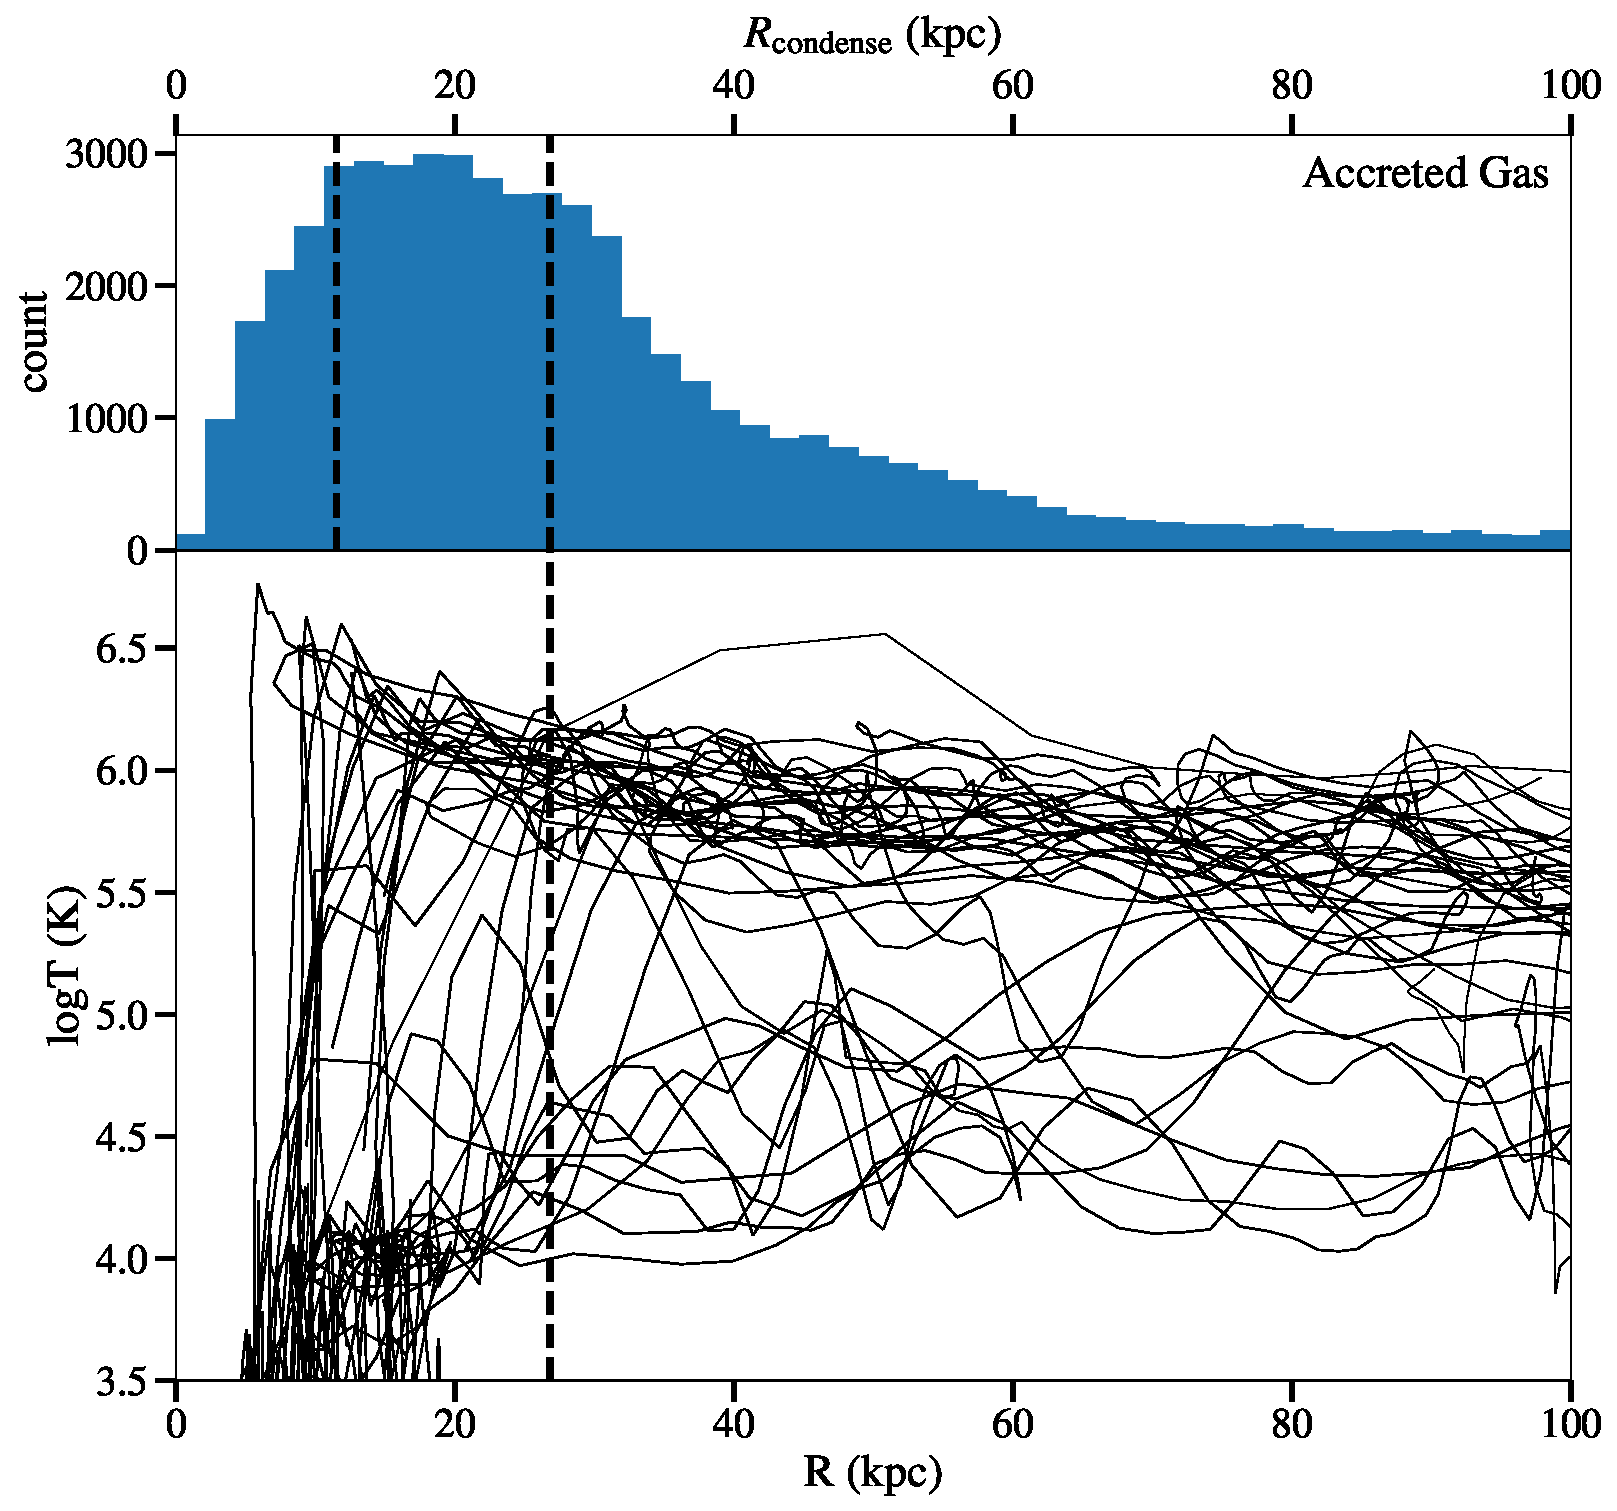
\includegraphics[width=\columnwidth]{figures/rcondense_and_tracks.pdf}
    \caption{
    Main panel: 50 T vs.\ R tracks, with sequential color indicating time or time minus accretion time . no median;
    Top panel: distribution of $\Rcool$
    \textbf{Add all particles with $R_{T=10^5\K}>100$ to $R=100$ bin, so we don't ignore them}
    \textbf{Is this only m12i? lets see same plot for other sims (maybe not eventually to go into paper).}
    \textbf{Add another panel with K vs.~R for the same particles.}
    \textbf{Add in coloring by $t - t_{\rm{condense}}$.}
    \textbf{Make y-axis T but in log space (not log T).}
    \textbf{Add label to 0.1$R_{\rm vir}$.}
    \textbf{Make upper panel less tall, so its clear its an addendum to the bottom panel}
    }
    \label{f: T vs R}
\end{figure}

\begin{figure}
    \centering
    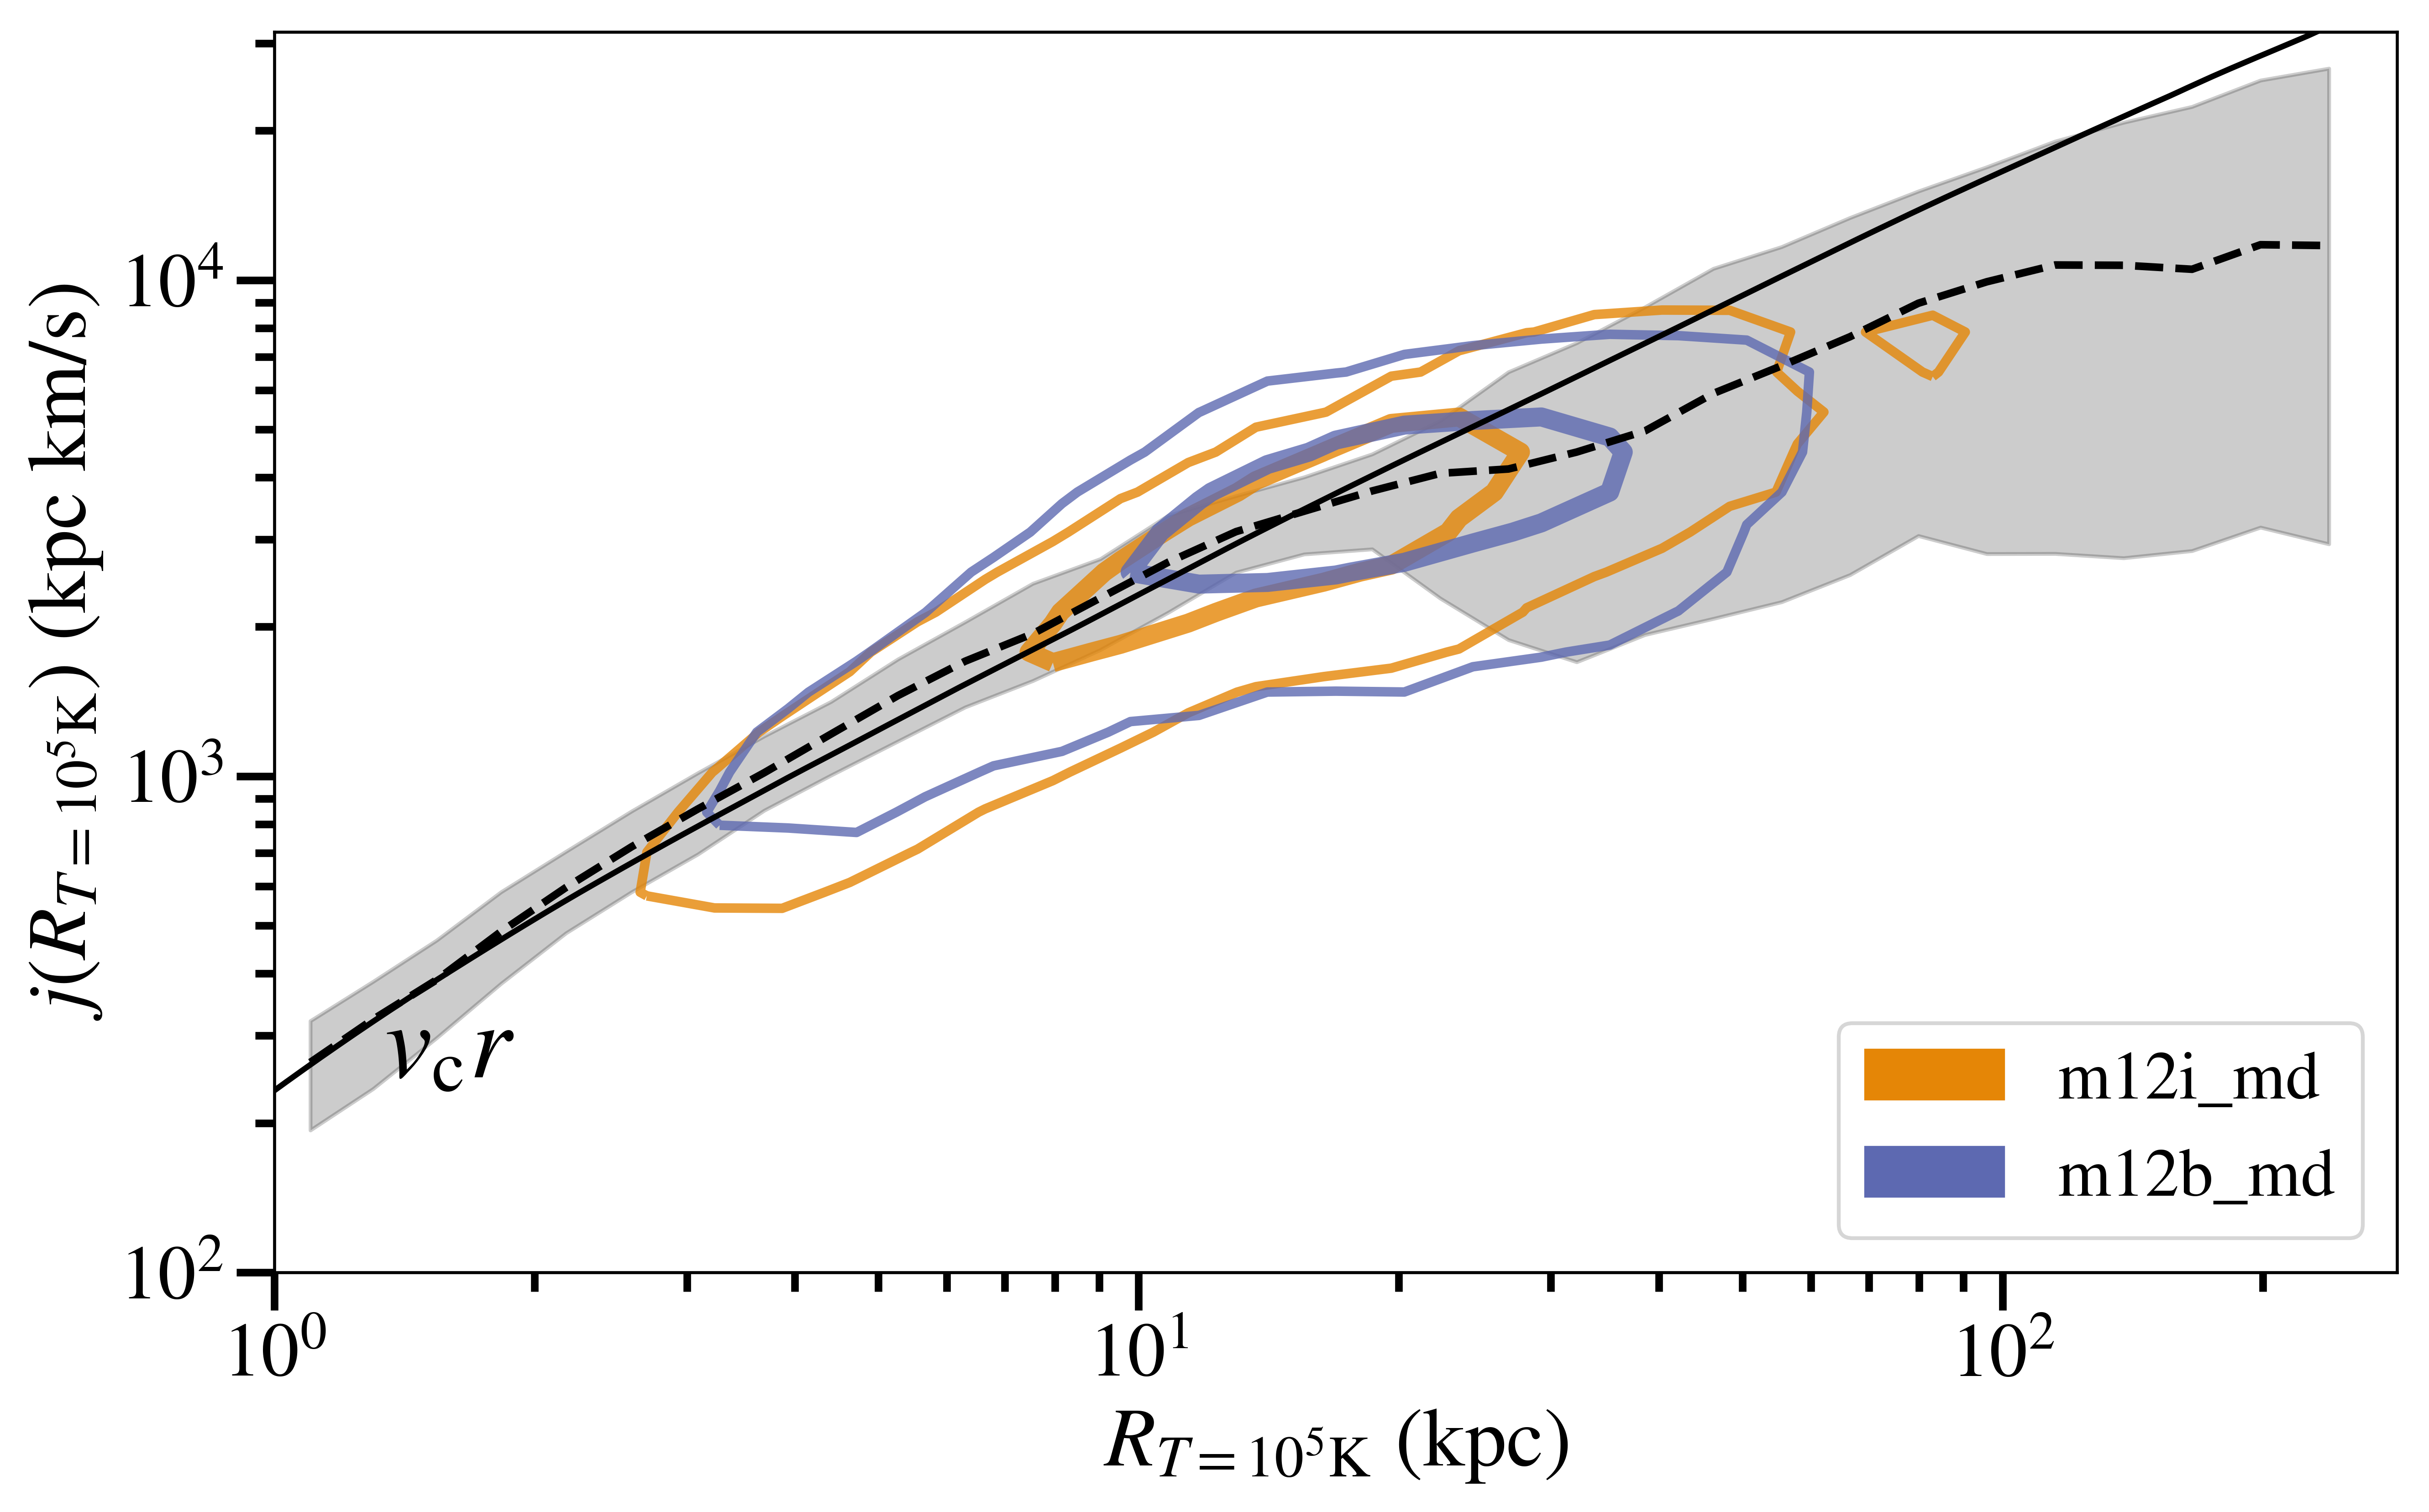
\includegraphics[width=\columnwidth]{figures/j_vs_rcondense.png}
    \caption{
    Distribution of $\Rcool$ vs j($\Rcool$) for four FIRE-2 halos with $L(z=0) \sim L^\star$.
Thick (thin) contours enclose values for 50\% (90\%) of the accreted gas particles.
The angular momentum as a function of radius for all gas in \texttt{m12i} at $z=0$ is displayed as a dashed line (the median) and shaded regions (5th-95th percentiles).
\textbf{The contours appear to match well with the circular velocity, but in reality so does the angular momentum of all gas at $z=0$, it's just that there are many order of magnitude on the y axis. In fact, the angular momentum of all gas at $z=0$ matches better, maybe??}
\textbf{Maybe add in a line that indicates the angular momentum necessary for full support?}
\textbf{Does the 100 kpc-cooling gas only occur in simulations without metal diffusion? If so, is it seen for particularly metal-enriched particles?}
\textbf{Is the 100 kpc-cooling gas related to satellite galaxies?}
\textit{
In all halos the distributions are consistent with $j_{\rm c} = v_{\rm c} r$, i.e. gas cools once circularized.
This demonstrates that the variable angular momentum of incoming gas drives the width in the $\Rcool$ distribution.
}
    }
    \label{f:Rcool}
\end{figure}

\begin{figure}
    \centering
    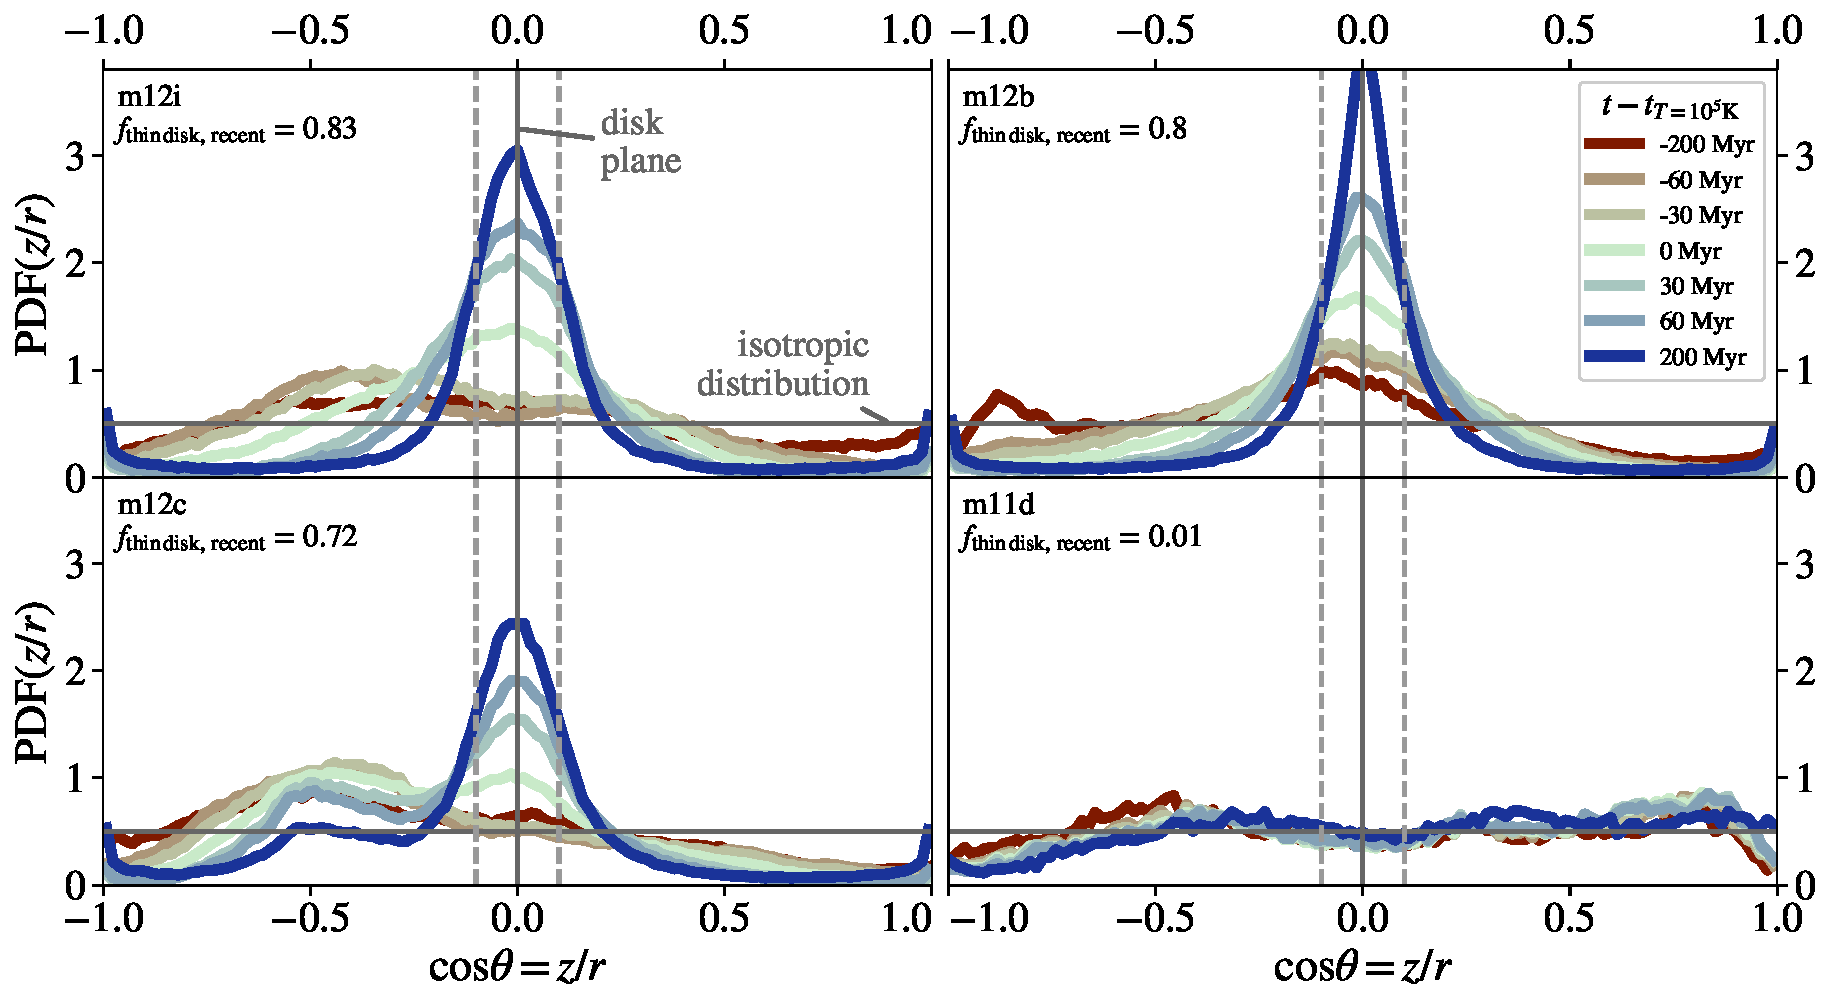
\includegraphics[width=\columnwidth]{figures/theta_vs_t.pdf}
    \caption{
    Angular distribution of accreting gas over 250 Myr before/after cooling.
    Prior to cooling the gas is distributed without a strong preferential direction (as shown by the consistency with the horizontal line representing a spherical PDF).
    After cooling the gas is primarily found in the disk at $\cos\ \theta = 0$.
    }
    \label{f: theta vs R}
\end{figure}

% Distribution of r1e5
\textit{
Isotropic cooling occurring randomly within $R_{\rm vir}$ would cool in a wide distribution with a median at $0.8 R_{\rm vir}$, while for our accreted gas the median $\Rcool \approx 0.06 R_{\rm vir}$.
}

\begin{figure}
    \centering
    % \includegraphics{}
    \caption{cooling emission in X-ray, optical and UV lines vs.\ radius, only from tracked particles}
    \label{f:emission}
\end{figure}

\section{Discussion}

\textbf{
We should make it clear why the gas cools so quickly at the angular momentum radius when the definition of inner CGM virialization is $t_{\rm cool} > t_{\rm ff}$.
This could be a point of confusion for the readers (it at least is for me).
Is it due to pile-up of material, increasing density and driving cooling?
}

\subsection{AGN feedback}

\begin{itemize}
    \item Results expected to be valid after disc forms (Paper III) and before AGN feedback kicks in (ref.~Byrne+)
    \item Results are baseline for detecting effects of feedback in observations / simulations
    
\end{itemize}
\subsection{Contrast with Precipitation}

\textbf{We should note that we may lack the resolution necessary to see true precipitation.}

\section{Conclusions}

\textbf{TBD.}

\section*{Acknowledgements}

\textbf{TBD.}


%%%%%%%%%%%%%%%%%%%%%%%%%%%%%%%%%%%%%%%%%%%%%%%%%%

%%%%%%%%%%%%%%%%%%%% REFERENCES %%%%%%%%%%%%%%%%%%

% The best way to enter references is to use BibTeX:

\bibliographystyle{mnras}
\bibliography{example} % if your bibtex file is called example.bib


% Alternatively you could enter them by hand, like this:
% This method is tedious and prone to error if you have lots of references
%\begin{thebibliography}{99}
%\bibitem[\protect\citeauthoryear{Author}{2012}]{Author2012}
%Author A.~N., 2013, Journal of Improbable Astronomy, 1, 1
%\bibitem[\protect\citeauthoryear{Others}{2013}]{Others2013}
%Others S., 2012, Journal of Interesting Stuff, 17, 198
%\end{thebibliography}

%%%%%%%%%%%%%%%%%%%%%%%%%%%%%%%%%%%%%%%%%%%%%%%%%%

%%%%%%%%%%%%%%%%% APPENDICES %%%%%%%%%%%%%%%%%%%%%

\appendix

\section{Some extra material}

If you want to present additional material which would interrupt the flow of the main paper,
it can be placed in an Appendix which appears after the list of references.

%%%%%%%%%%%%%%%%%%%%%%%%%%%%%%%%%%%%%%%%%%%%%%%%%%


% Don't change these lines
\bsp	% typesetting comment
\label{lastpage}
\end{document}

% End of mnras_template.tex